%%%%%%%%%%%%%%%%%%%%%%%%%%%%%% -*- Mode: Latex -*- %%%%%%%%%%%%%%%%%%%%%%%%%%%%
%% thesis-ch1.tex --
%% Author          : Robert Brewer
%% Created On      : Fri Sep  5 13:50:18 1997
%% Last Modified By: Philip M. Johnson
%% Last Modified On: Fri Oct 10 09:06:11 2003
%% RCS: $Id: thesis-body.tex,v 1.4 2000/03/17 21:28:10 rbrewer Exp $
%%%%%%%%%%%%%%%%%%%%%%%%%%%%%%%%%%%%%%%%%%%%%%%%%%%%%%%%%%%%%%%%%%%%%%%%%%%%%%%
%%   Copyright (C) 1998 Robert Brewer
%%%%%%%%%%%%%%%%%%%%%%%%%%%%%%%%%%%%%%%%%%%%%%%%%%%%%%%%%%%%%%%%%%%%%%%%%%%%%%%
%%

\chapter{Introduction}

This is the start of my thesis.  In this thesis, I intend to:

\begin{enumerate}
\item Explore the mysteries of the universe.
\item Go where no CSDL graduate student has gone before.
\end{enumerate}

Here is a figure that shows how to include figures:

In Figure \ref{fig:hackystat2}, I illustrate how to include figures.

\begin{figure}[htbp]
  \centering
  \includegraphics[width=1.0\textwidth]{figs/hackystat2.jblanket.package.eps}
  \caption{Summary view of JBlanket report for Hackystat version 2}
  \label{fig:hackystat2}
\end{figure}

Also, no thesis would be complete without a citation \cite{csdl2-03-01}.

